\section{Introduction}
\label{sec:intro}

\begin{figure}[t]
\centering
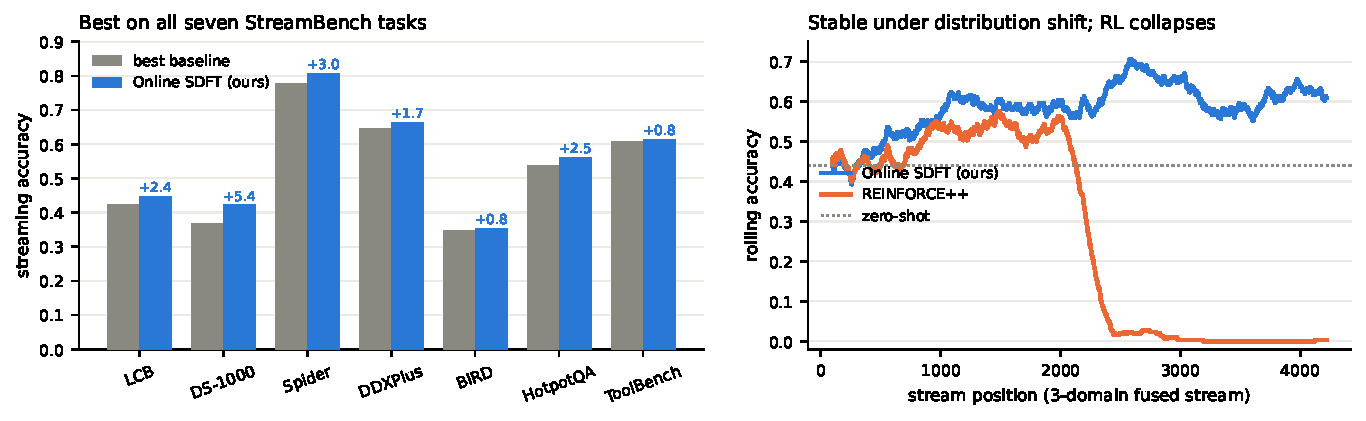
\includegraphics[width=\linewidth]{figures/fig1.pdf}
\caption{\textbf{Left:} final streaming accuracy on seven StreamBench tasks;
\method{} (blue) exceeds the strongest baseline (zero-shot, Self-StreamICL, or
REINFORCE++, gray) on every task. \textbf{Right:} rolling accuracy on a
4{,}219-problem stream interleaving three domains; \method{} improves throughout
while REINFORCE++ collapses after roughly 2{,}000 problems.}
\label{fig:headline}
\end{figure}

A language model deployed as an agent meets its work as a stream. A coding
assistant sees one issue after another, and each resolved ticket reveals whether
its patch passed the tests. The feedback is sparse, a single verified bit per
attempt, but it is grounded and it arrives continuously. Deployed models are
nevertheless frozen: a mistake made on Monday is repeated on Friday, because
nothing connects the stream of verified outcomes back to the weights.

Two research programs address parts of this problem. The first improves models
between deployments. Self-training methods sample from the model, keep outputs
that pass a correctness check, and fine-tune on the survivors
\citep{zelikman2022star, gulcehre2023rest, singh2024beyond, yuan2023scaling};
reinforcement learning from verifiable rewards scales the same signal to
emergent reasoning \citep{shao2024deepseekmath, guo2025deepseekr1}. These loops
need the task corpus up front and make several generation and training sweeps
over it, so they cannot run while the stream is being served. The second
program adapts agents during deployment but avoids weight updates: verified
experiences go into buffers, skill libraries, and playbooks that are retrieved
into the prompt \citep{shinn2023reflexion, wang2024voyager, zhao2024expel,
wang2025agent, madaan2022memprompt, zhang2025agentic}, the design StreamBench
\citep{wu2024streambench} adopted for streaming evaluation. Under this design
the model itself never improves. Gains are capped by the frozen base, disappear
without the memory, and retrieval can hurt when neighbors mislead
(\S\ref{sec:exp-bench}). Test-time training does update weights but discards
them after each instance \citep{sun2020ttt, akyurek2025surprising,
hubotter2025sift}. Applying rollout-batch RL to the streaming bit is also
problematic: policy-gradient methods are prone to entropy collapse on long
horizons even offline \citep{cui2025entropy, liu2025prorl}, and in our
experiments a stability-oriented variant \citep{hu2025reinforcepp} diverges on
a long mixed-domain stream.

What is missing is a stable online learning rule that turns each verified
success into a permanent weight update at the moment it happens. Our starting
point is a simple observation: \textbf{a model conditioned on its own
oracle-verified answer is a teacher for the same model without it.} Matching
the teacher's next-token distribution, with a forward KL against a frozen base
reference, moves the answer's information into the weights in a small and
verified step. We build \method{} around this rule. Verified answers enter a
reward-filtered memory \citep{wu2024streambench} that serves two purposes:
retrieval of demonstrations for the current problem, and hints for
distillation. Because a single greedy pass would only ever train on problems
the model already solves, a forward re-evaluation step retries recent failures
with the current model, which converts weight gains into new verified data.
Scoring always precedes any use of a problem for training, so the streaming
metric remains strictly predict-then-train.

We evaluate on seven StreamBench tasks and two stress tests.
\begin{itemize}
\item \textbf{Streaming accuracy} (\S\ref{sec:exp-bench}): \method{} reaches
  the best accuracy on all seven tasks against zero-shot, Self-StreamICL, and
  REINFORCE++ baselines, including tasks where retrieval-ICL falls below
  zero-shot.
\item \textbf{Distribution shift} (\S\ref{sec:exp-fused}): on a 4{,}219-problem
  stream interleaving three domains, one \method{} model matches or beats three
  per-domain specialists, with a $+3.4$-point gain on code relative to its own
  specialist. Retrieval stays within-domain for 99.9\% of queries, so this
  transfer is carried by the weights. REINFORCE++ diverges after roughly
  2{,}000 problems on the same stream.
\item \textbf{Online vs.\ batch} (\S\ref{sec:exp-transfer}): with loss, data,
  model, and oracle budget held fixed, streaming training beats batch
  self-distillation on source mastery; an exploration-augmented batch variant
  narrows the gap, isolating coverage as the main mechanism
  \todo{and transfer to an unseen domain as the remaining open comparison
  (runs in progress)}.
\item \textbf{Ablations} (\S\ref{sec:exp-ablations}): the gains are not
  explained by oracle budget, hint-conditioned generation, or sample count.
\end{itemize}
We are not aware of prior work that performs verified, weight-updating
self-distillation online over a deployment stream. The closest neighbors are
SDPO, which uses self-distillation inside rollout-batch RL \citep{hue2026sdpo};
offline SDFT, which requires a gold dataset \citep{yang2024selfdistillation};
and test-time methods whose updates are transient \citep{akyurek2025surprising}
or driven by unverified consensus rewards \citep{zuo2025ttrl}. Code,
per-problem logs, and a causal-ordering leakage audit are released.
